\normaltrue
\correctiontrue

%\UPSTIidClasse{11} % 11 sup, 12 spé
%\newcommand{\UPSTIidClasse}{12}

\exer{Mouvement T -- $\star$ \label{B2:13:01}}
\setcounter{numques}{0}
\UPSTIcompetence[2]{C2-05}
\UPSTIcompetence[2]{B2-13}
\index{Compétence C2-05}
\index{Compétence B2-13}
\index{Mécanisme à 1 translation}
\ifcorrection
\else
\textbf{Pas de corrigé pour cet exercice.}
\fi

\ifprof
\else
Soit le mécanisme suivant. On note $\vect{AB}=\lambda(t)\vect{i_0}$.
\begin{center}
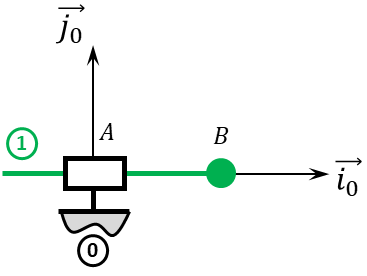
\includegraphics[width=.6\linewidth]{01_T_01}
\end{center}
\fi

\question{Quel est le mouvement de \textbf{1} par rapport à~\textbf{0}.}
\ifprof~\\
\textbf{1} est en translation de direction $\vi{0}$ par rapport à \textbf{0}.
\else
\fi

\question{Donner l'équation paramétrique de la trajectoire du point $B$, point appartenant à \textbf{1} par rapport à ~\textbf{0}.}
\ifprof~\\
On a $\vect{AB}=\lambda(t)\vect{i_0} $. La trajectoire du point $B$ est donc donnée par 
$\left\{ 
\begin{array}{l}
x_B(t) = \lambda (t) \\
y_B(t) = 0 \\
z_B(t) = 0 \\
\end{array}
\right.$ dans le repère $\repere{A}{i_0}{j_0}{z_0}$.
\else
\fi


\ifprof
\else

\footnotesize
\begin{center}
\begin{tabular}{|p{.9\linewidth}|}
\hline
Indications :
\begin{enumerate}
\item .
\item $x_B(t) = \lambda (t)$.
\end{enumerate} \\ \hline
\end{tabular}
\end{center}
\normalsize

\begin{flushright}
\footnotesize{Corrigé  voir \ref{B2:13:01}.}
\end{flushright}%
\fi


